\section{Prior Work in Manipulation Planning with Dynamics}

Higher-order constraints such as joint torques and end-effector accelerations can be addressed through several approaches that range from ``plan-and-filter'' methods which post-process geometric paths \cite{abderezaei2024clutter,kuntz2019fast} to kinodynamic planners that directly incorporate dynamics during planning \cite{li2016asymptotically,nayak2022bidirectional}.
Broadly there are four different approaches (\cref{fig:other-prior-work}). The literature is vast so we focus our approaches on manipulation tasks which involve the consideration of environment or object dynamics in addition to robot dynamics.

% \begin{figure*}
  \centering
    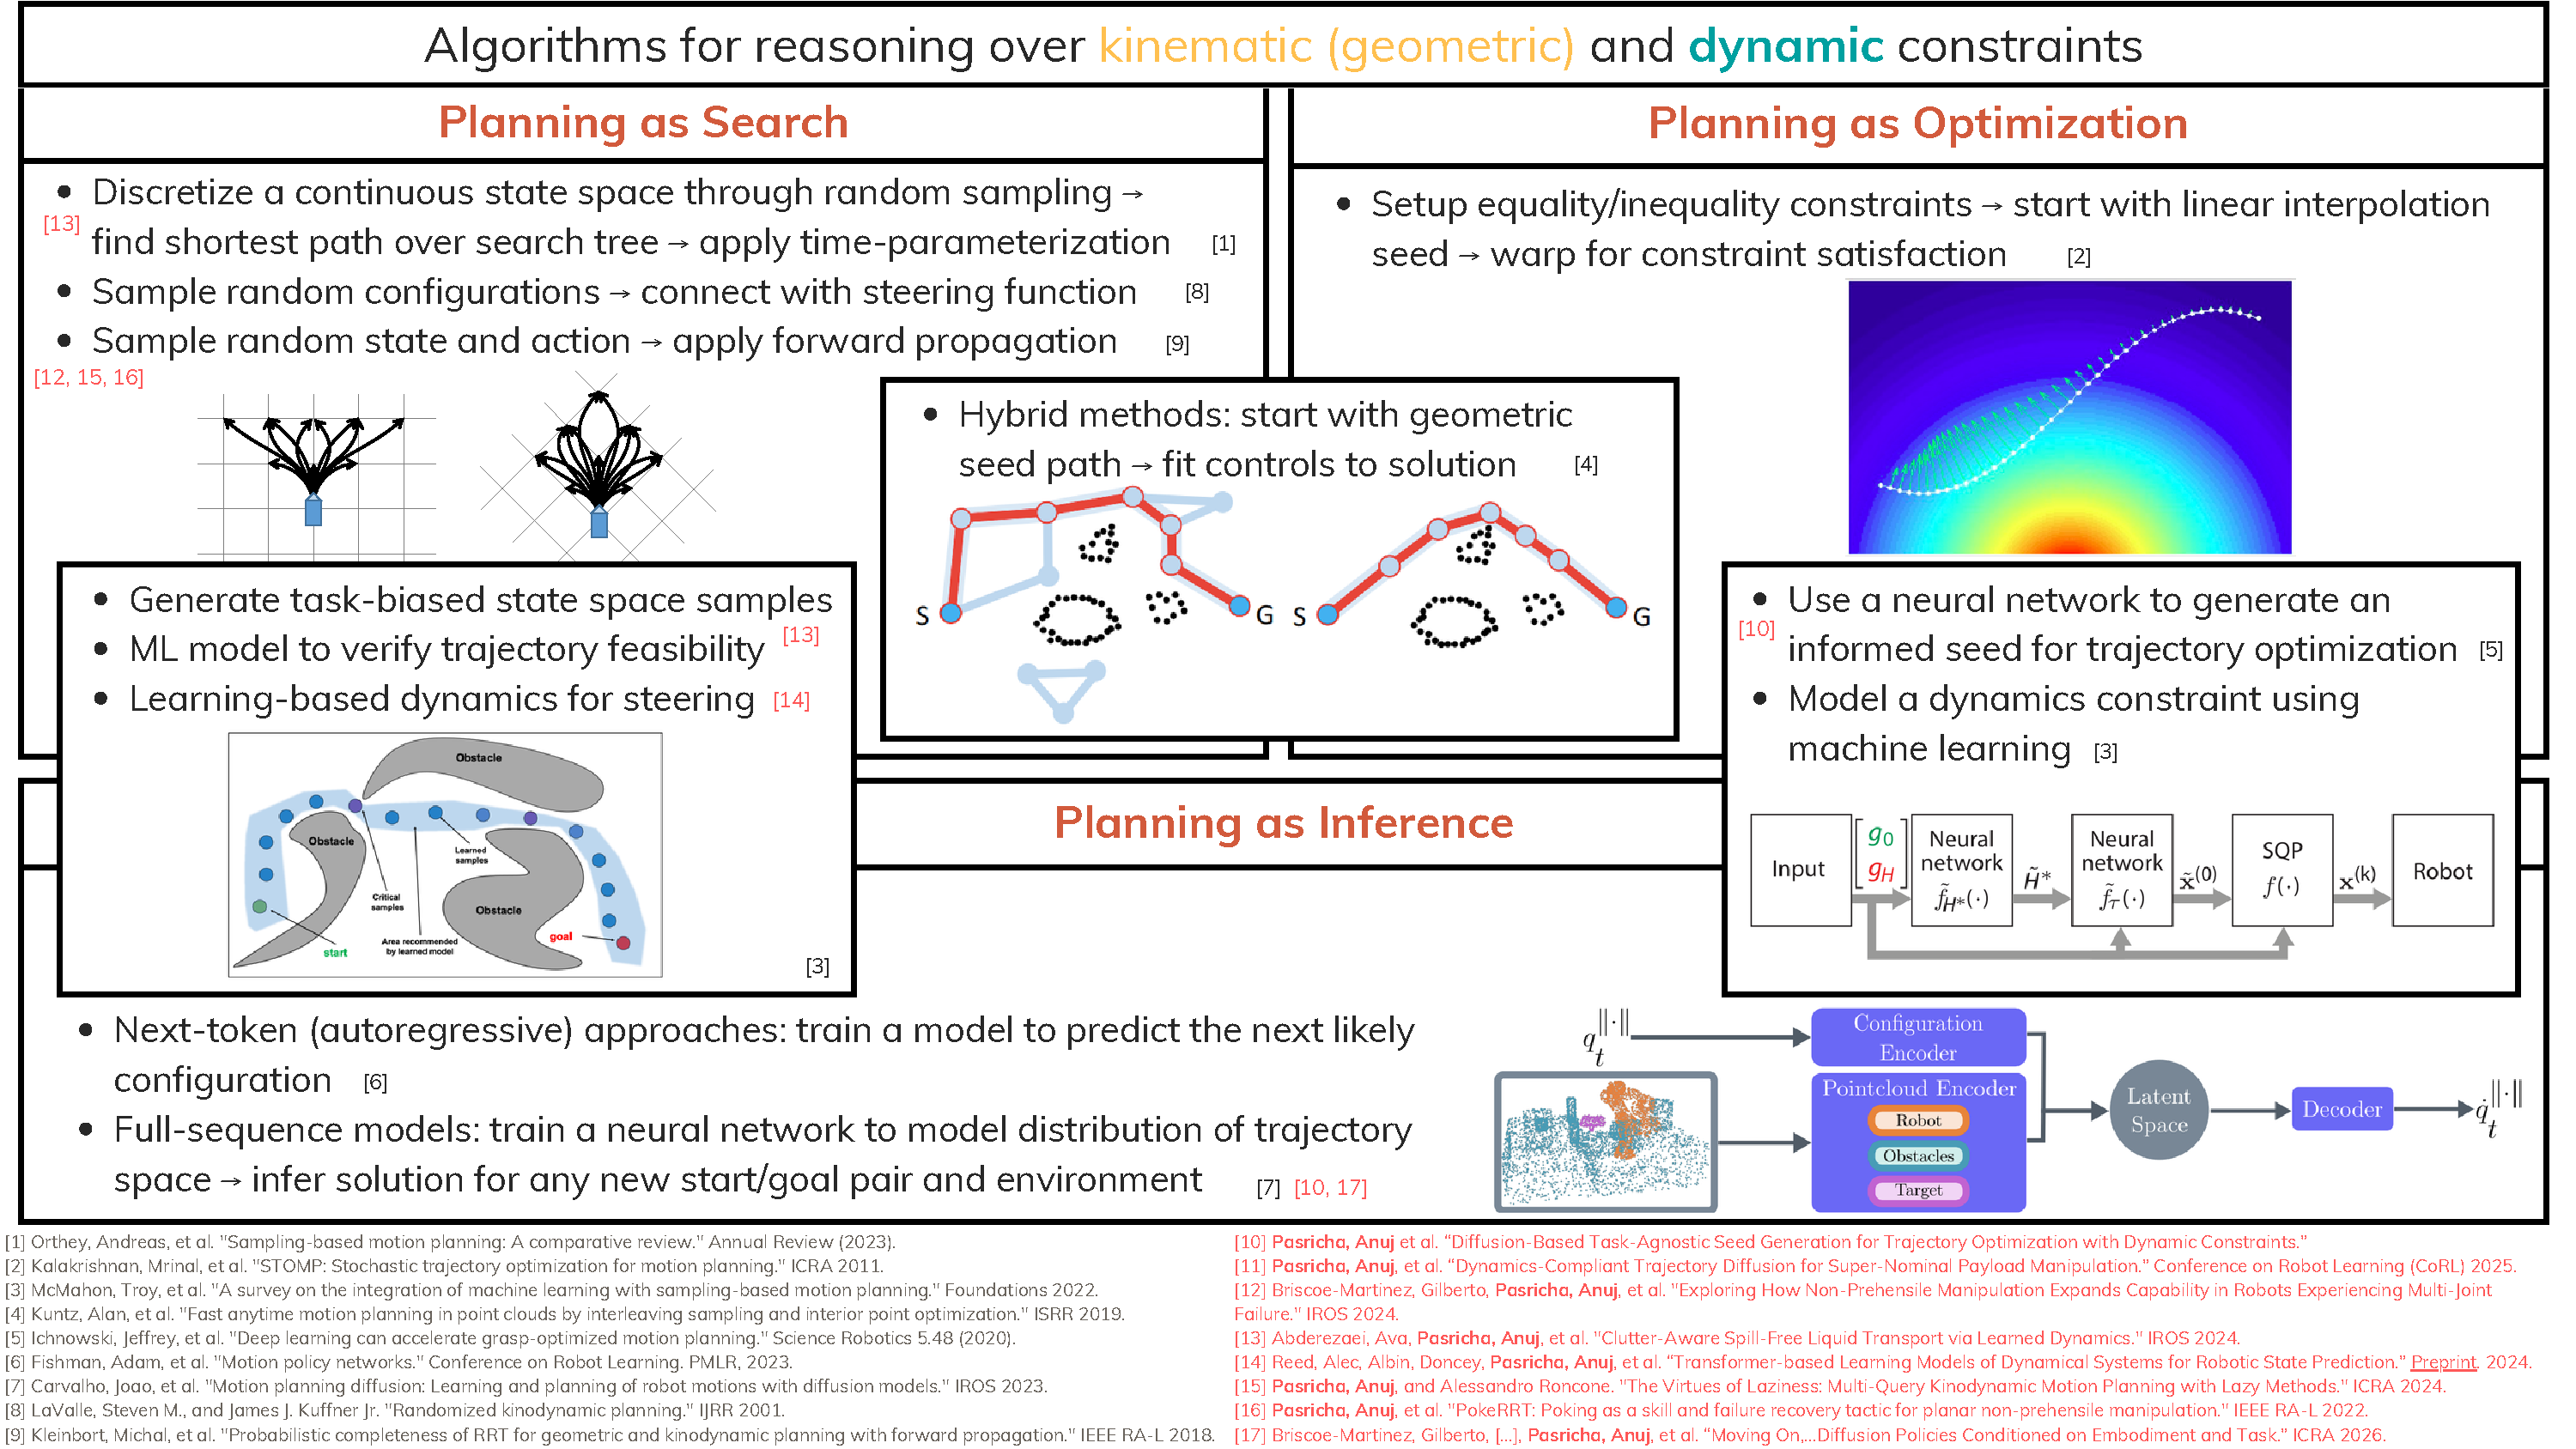
\includegraphics[width=\textwidth]{ThesisFilePkg/figs/prior.pdf}
  \caption{Motion planning approaches for robotic manipulation with kinematic and dynamic constraints span three broad categories: search, optimization, and inference, with hybrid methods existing at each of their intersections.}\label{fig:other-prior-work}
\end{figure*}

\header{Planning as Search}
At its very basic, this class of methods involves finding a configuration-space path is generated to satisfy geometric constraints including collision avoidance and joint limits \cite{orthey2023sampling}. Subsequently, time parameterization is applied---through bang-bang control or optimization techniques---to minimize traversal time while respecting velocity and acceleration constraints \cite{pham2018new,berscheid2021jerk}. The resulting trajectory is then evaluated against environmental dynamic constraints \cite{gaz2019dynamic}. This sequential process iterates until identifying a trajectory that successfully enables the desired dynamic robot-object interaction.
Although modular in nature which allows for the tuning of each component, this sequential framework may yield sub-optimal solutions and be computationally inefficient due to iterative refinement cycles when trajectories fail to satisfy all constraints, particularly when environmental models are inaccurate or constraints are too restrictive.

Kinodynamic planning simultaneously considers robot and object dynamics through interleaved state space exploration and control propagation. Many approaches employ steering functions (inverse models) to connect states. Examples include DIMT-RRT's quadratic steering function that obeys joint acceleration limits and non-zero initial and goal velocities \cite{kunz2014probabilistically}, AVP's computation of reachable velocities along a geometric path \cite{pham2013kinodynamic,johnson2012optimal}, and LQR-RRT*'s linearized dynamics with quadratic cost functions \cite{perez2012lqr,caldwell2018fast}. Alternatively, forward control propagation methods use random states and actions to construct dynamically feasible trees \cite{pasricha2022pokerrt}. SyCLoP and KPIECE guide exploration via state space discretization \cite{plaku2010motion,sucan2011sampling}, while SST optimizes paths through pruning and heuristic biasing \cite{li2016asymptotically}. GBRRT and GABRRT employ multiple propagation methods with bidirectional search \cite{nayak2022bidirectional}. Other techniques pre-map valid motions and search discretized state and control spaces \cite{shome2021asymptotically,bordalba2018randomized}. Despite theoretical completeness guarantees under certain conditions \cite{kleinbort2018probabilistic}, these methods face practical limitations in high-dimensional manipulation spaces and exhibit high variance in planning times, particularly when dealing with uncertainty and planning near operational limits \cite{kingston2018sampling}.

\header{Optimization-Based Approaches}
Optimization-based methods naturally integrate dynamics constraints by framing motion planning as the minimization of objective functions (e.g., smoothness, time optimality) subject to equality and inequality constraints that enforce collision avoidance, robot limitations, and dynamic feasibility \cite{kalakrishnan2011stomp,schulman2013finding,park2012itomp,ichnowski2020gomp}.
Typically formulated as quadratic programs, these approaches guarantee constraint satisfaction but demonstrate high sensitivity to initialization quality. This dependency has prompted the development of hybrid methodologies that bootstrap the optimization process with sampling or learning-based initializations \cite{ichnowski2020deep,kuntz2019fast,yan2024impact}. These integrated approaches leverage the strengths of both paradigms: the exploration capabilities of sampling/learning methods for identifying promising trajectory seeds, and the precision of optimization for refining solutions to satisfy strict dynamic constraints.
Optimal control formulations for dynamics-aware manipulation also exist \cite{arrizabalaga2024slosh,kim2014catching}. Despite their theoretical rigor, they face practical limitations in handling complex constraints and achieving reliable convergence for real-world manipulation problems.

\header{Learning-Based Approaches}
Finally, learning-based approaches offer promising directions for both generalizability and efficient trajectory generation while respecting system dynamics. Autoregressive models implicitly encode dynamics through dataset design \cite{fishman2023motion,qureshi2020motion}, while recent diffusion-based approaches provide non-autoregressive alternatives with improved sampling diversity \cite{carvalho2023motion,saha2024edmp}. Task-level diffusion policies, conditioned on language and visual embeddings \cite{ajay2023is,chi2023diffusionpolicy}, demonstrate potential for generating diverse behaviors from high-level task specifications.
While these approaches yield impressive real-world behaviors, provide continual improvement over deployment lifespan, and avoid explicit state space exploration for each new query, they typically focus on position-controlled tasks and grasping-based manipulation and incur significant training and data acquisition costs.

% \begin{figure*}
  \centering
    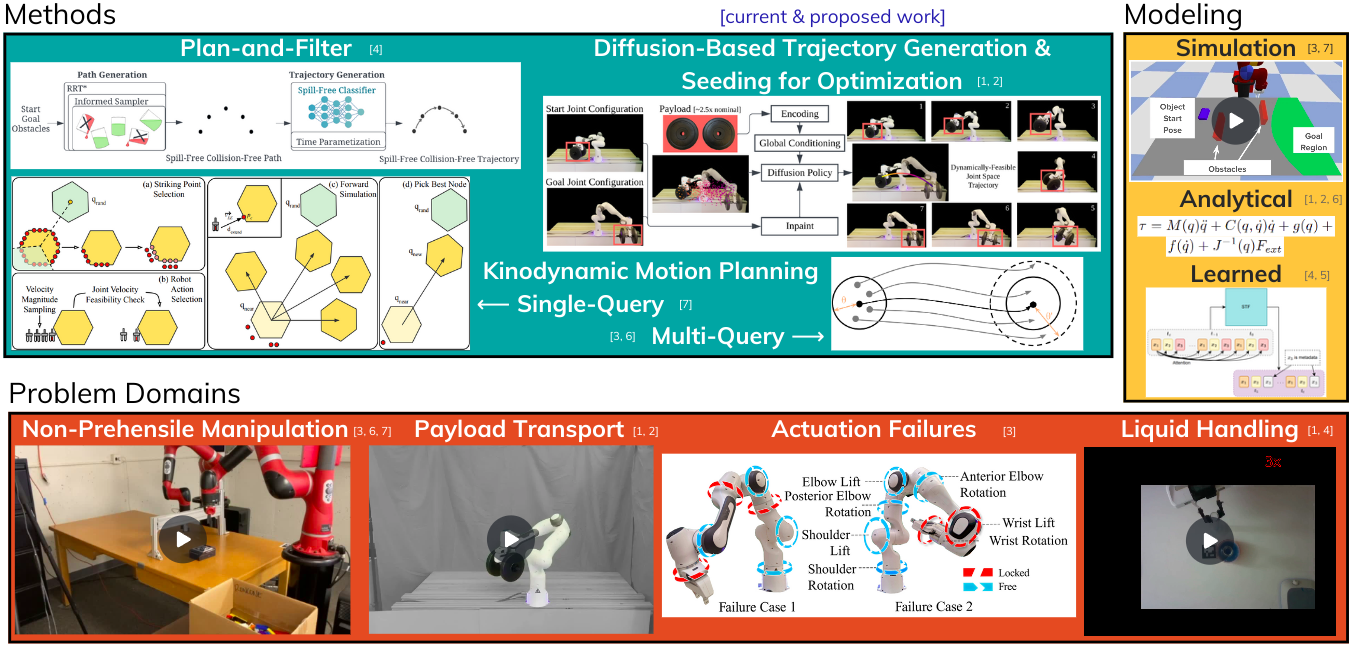
\includegraphics[width=\textwidth]{figs/my-work.png}
  \caption{My prior, current, and proposed work progress from sampling-based kinodynamic planning to diffusion-based trajectory generation, leveraging various modeling approaches applied to a broad class of manipulation problems that are subject to both kinematic and dynamic constraints.}\label{fig:my-work}
\end{figure*}

\header{Hybrid Approaches}
Hybrid approaches can also exist at each intersection of the aforementioned methods and leverage the benefits of each to create a more robust system.
At the intersection of search-based and optimization-based methods, hybrid techniques typically begin with a seed path generated through sampling-based algorithms and subsequently fit controls to this solution \cite{kuntz2019fast}. This approach combines the exploratory advantages of search-based methods with the refinement capabilities of trajectory optimization.
In search-based planning, neural networks generate task-biased state space samples \cite{mcmahon2022survey}, while in optimization contexts, they provide informed seeds for trajectory optimization \cite{ichnowski2020deep}. This integration addresses the initialization sensitivity of pure optimization approaches while maintaining their convergence properties.

\ul{The confluence of all three paradigms---search, optimization, and inference---represents the frontier of motion planning research.}
Significant challenges remain in developing unified approaches that can reliably handle complex robot-object dynamics while maintaining computational efficiency and generalizability across multiple tasks---a gap my work directly addresses to enable a broad range of new capabilities beyond geometric reasoning alone.
